\chapter{Classical phase-sensitive ghost imaging}
In the previous chapter, we explored the benefits afforded by quantum OCT over classical OCT, finding that both axial resolution improvement and even-order dispersion cancellation originate not from quantum effects but rather from the phase-sensitive cross-correlations between the signal and idler beams in quantum OCT. We then constructed a classical phase-sensitive light source by using SPDC in the high-brightness regime, which we utilized to implement phase-conjugate OCT. Demonstration of phase-conjugate OCT allows us to use a classical light source and classical detection to realize the benefits of quantum OCT. However, there are other ways to construct classical phase-sensitive light sources.

In this chapter, we focus on the application of phase-sensitive light sources to ghost imaging, a transverse imaging modality that has been receiving considerable and increasing attention of late owing to its novel physical characteristics and its potential applications to remote sensing. Ghost imaging exploits the cross correlation between the photocurrents obtained from illumination of two spatially-separated photodetectors by a pair of highly-correlated, partially-coherent optical beams. One beam, referred hereinafter as the signal beam, interrogates a target (or sample) and then illuminates a single-pixel (bucket) detector that provides no spatial resolution. The other beam, which we refer to as the reference beam, does not interact with the target, but it impinges on a scanning pinhole detector or a high-resolution camera, hence affording a multi-pixel output. The term ``ghost imaging'' refers to the fact that neither photocurrent alone yields a target image, but cross-correlating the two photocurrents does produce an image of the object.  

A basic schematic of the ghost imaging concept is shown in Figure \ref{figure:ghost-schematic}. Pittman et al. realized the first such ghost imaging experiment \cite{pittman-ghost} using entangled pairs of signal and idler photons, with a bucket detector on one arm and a spatially-resolving detector on the other arm, showing that it was possible to image an object placed in the arm with no spatial resolution by counting the coincidences between the two detectors. At the time, this was interpreted as a quantum phenomenon, owing to the entanglement of the signal and idler photons. However, subsequent experiments by Valencia et al. \cite{valencia-two} and Ferri et al. \cite{ferri-high} demonstrated ghost imaging using pseudothermal light, obtained by illuminating a rotating ground-glass disk under laser light followed by a beam splitter. Abouraddy et al. analyzed the role of entanglement in several two-photon imaging configurations using quantum descriptions of the optical fields \cite{abouraddy-role,abouraddy-fourier}. The disparity between the theories of thermal-light ghost imaging experiments at the time, which use semiclassical descriptions of the field, and those using entangled photons, sparked numerous discussions about the advantages and unique properties of each \cite{dangelo-identifying,bennink-quantum,gatti-entangled}, and prompting development of a unified framework to describe the fundamental physics of ghost imaging.

Erkmen and Shapiro developed such a unified theory of ghost imaging with Gaussian-state light \cite{erkmen-unified} that encompasses both biphoton and pseudothermal light sources. In the case of SPDC, a nonclassical phase-sensitive cross correlation between the signal and idler photons is exploited to achieve the ghost image; in the case of pseudothermal light sources, it is the phase-insensitive cross correlation between the two arms as imposed by the ground glass diffuser that produces the ghost image. However, they also showed the possibility of using unconventional, classical phase-sensitive light sources to achieve ghost imaging. In this chapter, we implement such a system by using spatial light modulators (SLMs) to impose phase-sensitive correlations between the two arms.

In this chapter, we implement such a phase-sensitive classical source and demonstrate the first phase-sensitive classical ghost imaging experiment, and similar to PC-OCT, showing that phase-sensitive coherence is not unique to quantum sources.

\begin{figure}[htb]
\centerline{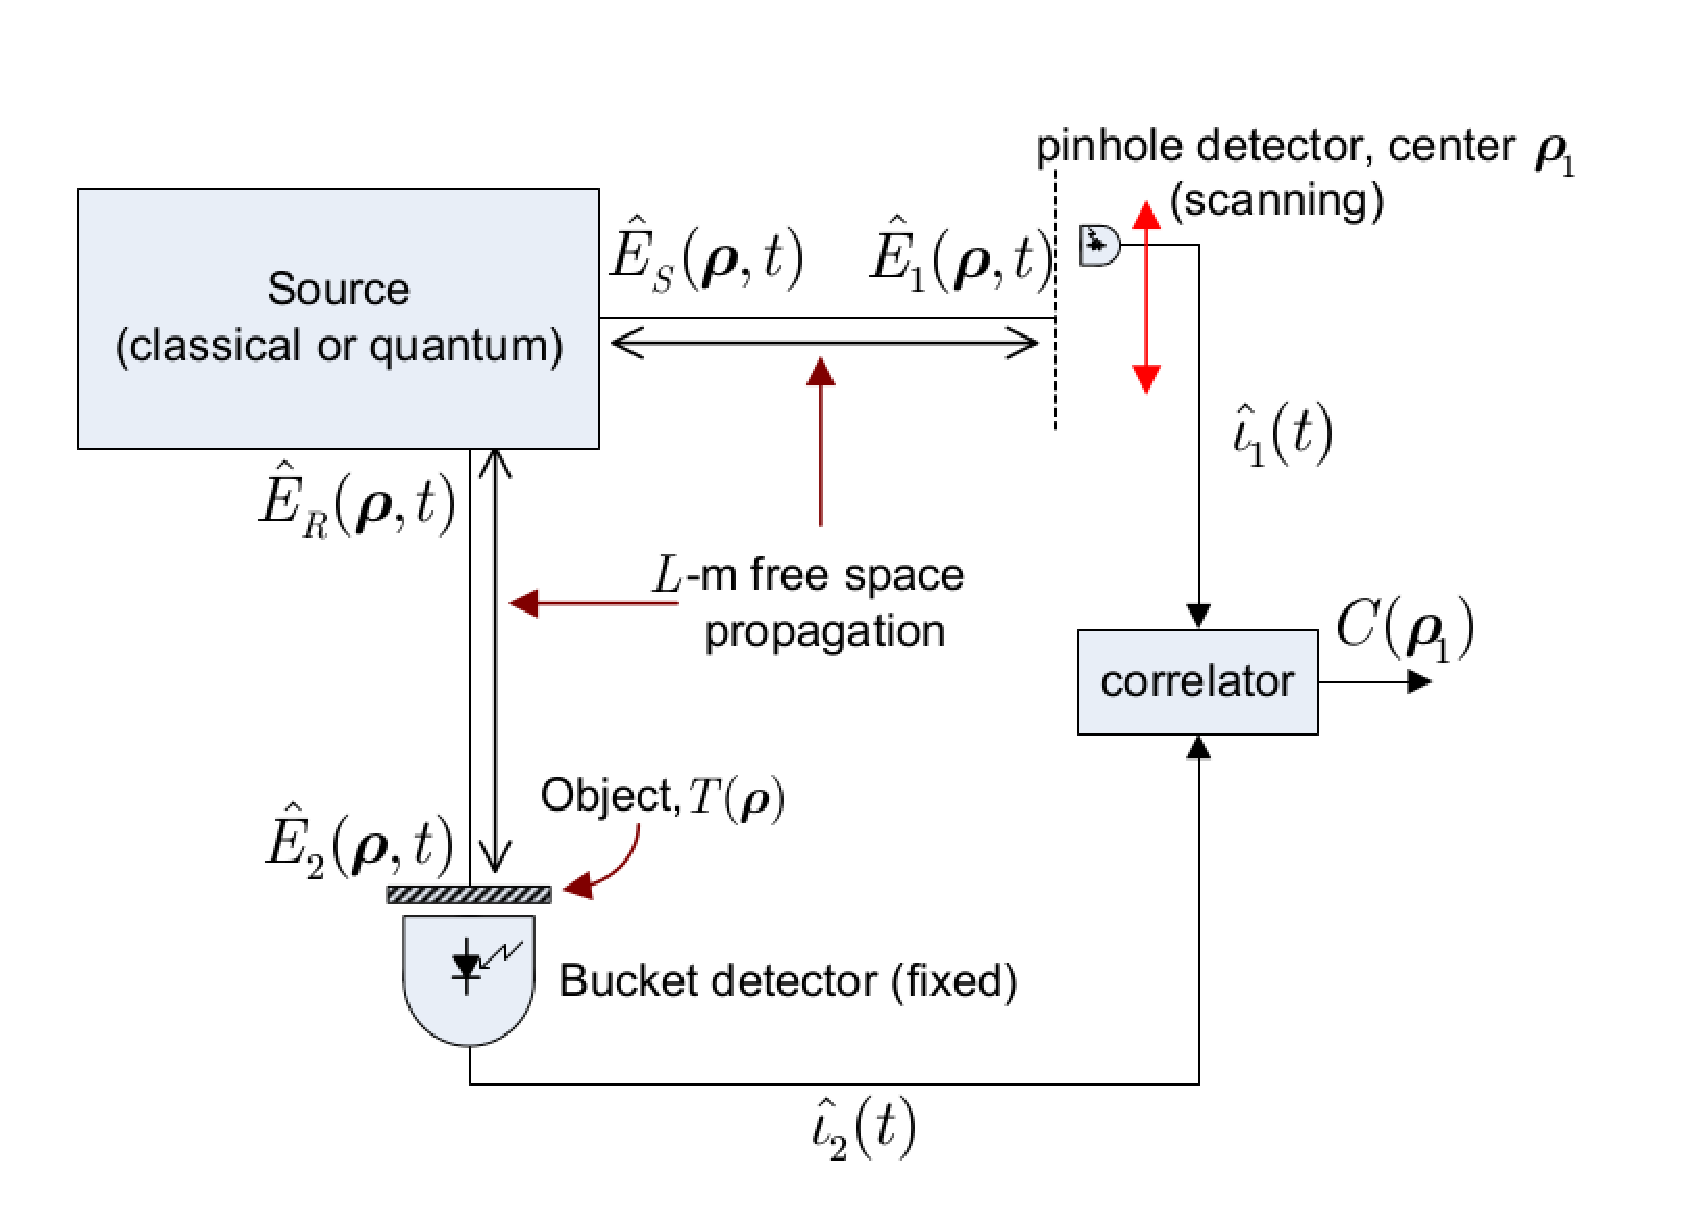
\includegraphics[width=12cm]{figure-ghost-schematic.pdf}}
\caption{Conceptual ghost imaging schematic, reproduced from Erkmen et al. \cite{erkmen-unified}.}
\label{figure:ghost-schematic}
\end{figure}

\section{Near- and far-field ghost imaging}

Erkmen and Shapiro extensively analyzed ghost imaging for the case of jointly-Gaussian signal and reference fields and explored both the near field, where diffraction effects are negligible, and far-field propagation where diffraction spread is dominant. For phase-insensitive coherence propagation, in which the phase patterns of the signal and reference fields are directly correlated (such as the signal and reference arms generated by a rotating ground glass followed by a beam splitter), the difference between near-field and far-field regimes is defined by a single Fresnel number,
\begin{equation}
D_0 = \frac{k_0 \rho_0 a_0}{2L}
\end{equation}
where $k_0$ is the laser light's wavenumber, $a_0$ is the source intensity radius, $\rho_0$ is its coherence radius, and $L$ is the propagation distance to the target, where $D_0 < 1$ indicates being in the far field and $D_0 > 1$ indicates being in the near field \cite{erkmen-unified}.

However, for phase-sensitive coherence propagation, in which the phases of the signal and reference beams are anticorrelated at the source plane, the near and far field regimes are defined by two Fresnel numbers: the Fresnel number for diffraction of the coherence length,
\begin{equation}
D_N = \frac{k_0\rho_0^2}{2L}
\end{equation}
and the Fresnel number for diffration of the intensity radius,
\begin{equation}
D_F = \frac{k_0 a_0^2}{2L}\,\,.
\end{equation}

For SLM-based ghost imaging, we assume low coherence where $\rho_0 < a_0$. In this case for phase-sensitive imaging the near-field regime is defined by $D_N > 1$ and the far-field is defined by $D_F < 1$, which is more stringent than the condition for phase-insensitive light \cite{erkmen-unified}.

Erkmen and Shapiro showed that for a transmission mask $T(\rho)$ used as an object, the phase-insensitive far-field ghost image signature is proportional to $|T(\rho)|^2$, whereas the phase-sensitive far-field ghost image signature is proportional to $|T(-\rho)|^2$ \cite{erkmen-unified}. Thus, for phase-insensitive light we obtain an upright ghost image whereas in the phase-sensitive case we obtain an inverted ghost image. The inverted far-field ghost image is also characteristic of ghost imaging with biphoton sources, which also produce only phase-sensitive cross correlations.


\section{Ghost imaging with spatial light modulators}

Similar to our work in PC-OCT described in the previous chapter, we now turn to the implementation of a classical source of signal and reference beams with phase-sensitive cross-correlations in multi-spatial modes that is suitable for ghost imaging. We achieved this behavior by splitting an ordinary continuous-wave laser beam using a 50-50 beam splitter and imposing computer-generated pseudorandom phase patterns using a pair of synchronized spatial light modulators. By imposing identical phase patterns on the two SLMs we obtained phase-insensitive cross-correlations; by using opposite phase patterns on the two SLMs we obtained phase-sensitive cross-correlations between the two beams.

\subsection{SLM: Principle of operation}

There are two main principles of operation that are presently used in phase-modulating SLMs: deformable mirrors, which selectively deform spatial regions over an optical wavelength, and liquid crystal arrays, which exploit electric-field dependent birefringence to impose a phase pattern. SLMs based on deformable mirrors (such as those sold by Boston Micromachines) are insensitive to the polarization of the input beam, may operate at very high modulation frequencies (often in the range of tens of kHz), but may suffer from much higher cross-talk between adjacent pixels because they are mechanically linked. On the other hand, those that are liquid-crystal based (such as those sold by Boulder Nonlinear Systems and Hamamatsu) suffer less cross-talk, but only modulate a single polarization axis and are limited to much slower speeds, typically no higher than 50-200 Hz. In this work, we used a liquid crystal-based Boulder Nonlinear Systems Model P512 SLMs which have 512$\times$512 pixels with individually addressable phases. The array size is 7.68$\times$7.68 mm with a pixel fill factor of 83.4\%.

\subsection{Pitfalls}

Tests on the P512 SLMs reveailed a number of nonidealities. First, although specified to have a maximum switching frequency of 10-30 Hz, we found that this is highly dependent on the phase stroke: while a smooth ramp from a phase of $0$ to $2\pi$ is accomplishable at upwards of 30 Hz, a sudden step transition from $0$ to $\pi$, for example, may require $\sim 0.3$ seconds to settle. Thus, for the purpose of implementing ghost imaging in which we imposed uniformly-distributed random phases, we chose to limit the frame rate to about 2 Hz. The limits of the SLM may in fact be better characterized by an analog bandwidth rather than a maximum switching frequency.

Second, the fill factor of the P512 SLMs is 83.4\%, with the behavior of the dead regions unspecified. Using a lens to image the SLM surface onto a camera and a polarizer for phase analysis, we found that the dead regions had high cross-talk with adjacent pixels, which may result from falloff from the electric field of the active regions of those pixels.

Third, although the voltage-to-phase calibration provided by Boulder Nonlinear Systems was reasonably accurate for the center region of the SLM, we found that the full SLM surfaces deviated from being flat by as much as a few wavelengths. Xun and Cohn also documented similar distortions in a Boulder Nonlinear Systems SLM \cite{xun-phase}. Although in principle a per-pixel calibration could be done, we mitigated this issue by using only the center 128$\times$128 pixels of the SLM where the calibration is reasonably consistent.

\begin{figure}[t]
\begin{center}
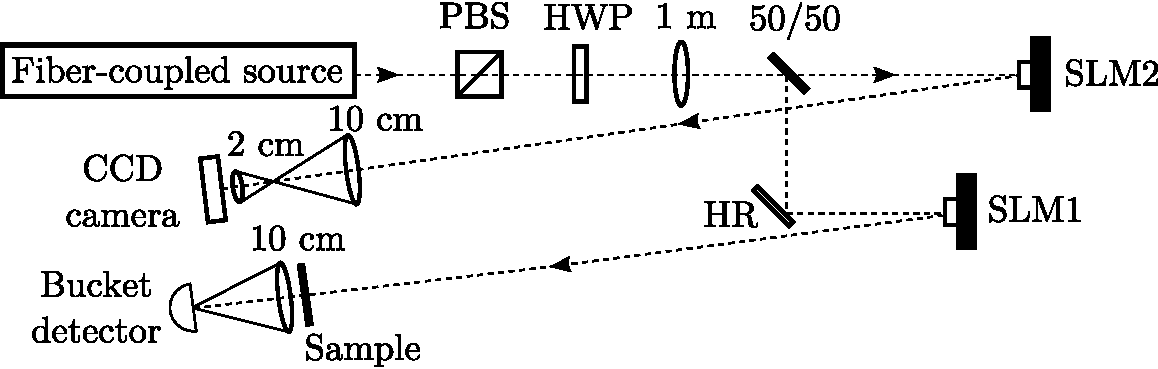
\includegraphics[width=13cm]{figure-ghost-setup.pdf}
\caption{Pseudothermal SLM-based ghost imaging setup that can be operated in either phase-sensitive mode (anti-correlated SLM phase patterns) or phase-insensitive mode (identical SLM phase patterns).}
\label{figure:ghost-setup}
\end{center}
\end{figure}


\section{Experimental setup}

Figure~\ref{figure:ghost-setup} shows our experimental setup.  A 10-mW, $\lambda_0$ = 795\,nm, laser beam was divided by a 50-50 beam splitter into signal and reference, each of which was focused to form a $w_0$ $\approx$ 200\,$\mu$m beam waist at its respective liquid-crystal SLM.  The polarizing beam splitter and half-wave plate ensured that the SLMs' illumination was vertically polarized. The SLMs (Boulder Nonlinear Systems) have 512$\times$512 pixels (each 15$\times$15 $\mu$m) with individually addressable phases. A control computer generated a 128$\times$128 array of uniformly-distributed random phases (on $[0, 2\pi]$) that were applied to the central 128$\times$128 pixels of SLM1 to modulate the signal beam with a $\rho_0$ = 7.5\,$\mu$m  coherence radius that is much smaller than $w_0$.  We programmed SLM2 synchronously with the same phase pattern as SLM1 for phase-insensitive cross-correlations, or with its complement for phase-sensitive light. We estimate a phase accuracy of $\sim$20 mrad for most cases, with a few small intervals (close to the zero phase end) where we were only able to successfully calibrate to within 50-100 mrad of precision. We generated and updated the SLMs' phase patterns at 2\,Hz. 

Theory \cite{erkmen-unified} shows that phase-sensitive and phase-insensitive correlations propagate differently, but $D_F \equiv \pi w_0^2/\lambda_0 L \ll 1$, with $L$ being the propagation distance, is sufficient for both to be in their far fields.  We used $L =80$\,cm from SLM1 to the object, so that $D_F \approx 0.2$, hence allowing a comparison of far-field phase-sensitive and phase-insensitive ghost images.  A 10-cm focal length, 5-cm diameter lens in the signal arm focused the light transmitted through the object on a standard photodetector. An identical 10-cm lens, placed in the reference arm $L = 80\,$cm from SLM2, served as the objective for a telescope with a 2-cm focal length eyepiece.  This telescope was adjusted to produce a $\sim$5.7$\times$ minified image of the speckle pattern at the objective plane. The camera was a shutterless Basler Pilot charge-coupled device (CCD) with 1600$\times$1200 pixels, each 7.4$\times$7.4\,$\mu$m in size with 12-bit dynamic range. We adjusted the CCD exposure and gain parameters to minimize the occurrence of vertical blooming \cite{janesick-astronomical}, which would degrade the image quality. Figure~\ref{figure:ghost-usaf}(a) displays a typical single-shot CCD image of the far-field speckle pattern in the reference arm produced by one of the random phase patterns at SLM2. The observed $\sim$1\,mm speckle radius at the objective lens is consistent with the expected far-field coherence radius, $\rho_L = \lambda_0 L/\pi w_0$. The expected spatial extent of the speckle pattern, set by the $2\lambda_0 L/\pi \rho_0 \approx 57$\,mm intensity diameter, is slightly larger than the 50-mm lens mount's circular aperture that is visible in Fig.~\ref{figure:ghost-usaf}(b).  

\begin{figure}[htb]
\centerline{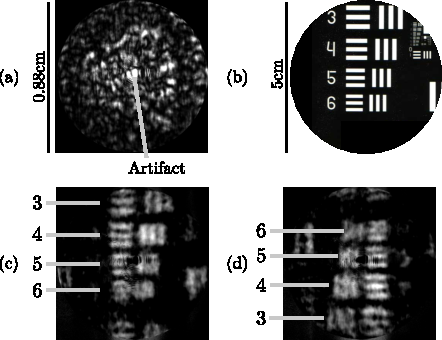
\includegraphics[width=12cm]{figure-ghost-usaf.pdf}}
\caption{(a) Sample single-frame speckle pattern as imaged by the CCD. The artifact in (a) is due to the SLMs' inter-pixel dead space. (b) Portion of a USAF spatial-resolution transmission mask used as the object. (c) Phase-insensitive and (d) phase-sensitive far-field ghost images, each averaged over 18640 realizations.}
\label{figure:ghost-usaf}
\end{figure}

The bright central spot in the Figure \ref{figure:ghost-usaf}(a) speckle pattern is an artifact that prevented ghost-image formation in that region.  We have traced the artifact to three potential problems in our experimental setup. First, the SLM phase patterns must be uniformly distributed over $[0,2\pi]$. Second, the polarization of the incident beam must exactly match the active axis of the SLM.  Any phase bias or polarization misalignment gives rise to a brighter center spot, but we were able to resolve these two problems by careful SLM calibration and polarization alignment, respectively. The third effect that we observed experimentally as well as confirmed by computer simulation, is that our SLMs are limited by a sub-optimal, $\sim$83\% pixel fill factor. The inter-pixel dead space behaves much like a 2-D diffraction grating, creating a grid of spots in the far field including a prominent zero-order spot at the center.

We used elements 3, 4, 5, and 6 from group 2 of a 1951 U.S.\ Air Force (USAF) resolution transmission test mask as our object, as shown in Fig.~\ref{figure:ghost-usaf}(b), and placed it just before the 10-cm lens in the signal arm.  The bucket detector and CCD outputs were fed in real-time to the control computer, which averaged the outputs from a sequence of SLM phase patterns to compute the cross-covariance between each CCD pixel and the bucket detector. Although the cross-correlation between the CCD pixels and bucket detector contains a high DC background which is present in classical-state ghost images \cite{erkmen-unified,erkmen-from}, we obtain a high-contrast ghost image of the object by computing the cross-covariance.


\section{Results}

Figures~\ref{figure:ghost-usaf}(c) and (d) show the measured phase-insensitive (in-phase SLMs) and phase-sensitive (anti-phase SLMs) ghost images of the test object, each obtained by averaging over 18640 random phase-pattern realizations. The only change made to the setup in transitioning from phase-insensitive to phase-sensitive ghost imaging was to switch the SLM1 and SLM2 patterns from in-phase (same phase) to anti-phase operation. The image inversion in the phase-sensitive case is in accord with theory \cite{erkmen-unified,erkmen-from} for phase-sensitive classical or quantum light sources.  Figure~\ref{figure:ghost-mitlogo} shows another example of image inversion between far-field phase-insensitive and phase-sensitive ghost imaging---here for an MIT-logo object---obtained using 7000 random phase-pattern realizations.

\begin{figure}[htb]
\centerline{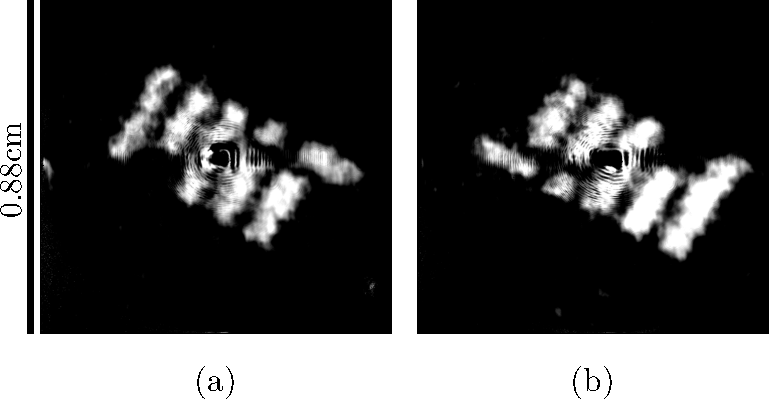
\includegraphics[width=12cm]{figure-ghost-mitlogo.pdf}}
\caption{MIT-logo ghost images after 7000 realizations for (a) 
phase-insensitive and (b) phase-sensitive light, showing image inversion in (b). The images are individually normalized, with the noise levels clipped for improved visibility. The bright-spot artifact at the center prevents us from obtaining an image in that small region.}
\label{figure:ghost-mitlogo}
\end{figure}

Figures~\ref{figure:ghost-usaf}(c) and (d) show comparable spatial resolutions for the phase-insensitive and phase-sensitive ghost images. The known spacings for the markings on the USAF test mask allow us to evaluate that resolution. In particular, the line spacings for elements 3 and 4 (the largest two elements) are well separated, but those for elements 5 and 6 are less discernible. We thus estimate the spatial resolution to be approximately equal to the spacing between lines in element 4, which is 1.42\,mm. This value is in good agreement with theory \cite{erkmen-unified}, which shows that the resolution is speckle-size limited to the object-plane spatial coherence radius $\rho_L \approx 1.0$\,mm.

\begin{figure}[htb]
\centerline{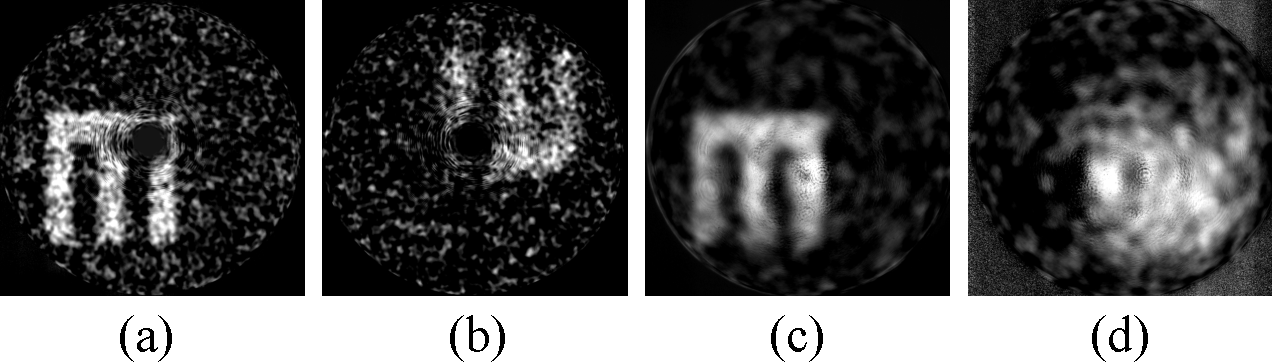
\includegraphics[width=14cm]{figure-ghost-blur.pdf}}
\caption{Far-field ghost imaging under loose focusing ($w_0$ = 150\,$\mu$m) for (a) and (b), and tight focusing ($w_0$ = 50\,$\mu$m) for (c) and (d), with the SLM located at a distance of 2.75$\times$ the Rayleigh range $z_R$. The mask is an off-center letter M.  
Phase-insensitive images in (a) and (c) are not affected, but 
phase-sensitive measurements in (b) and (d) show degradation that is severe for tight focusing in (d).}
\label{figure:ghost-blur}
\end{figure}

Our experiments showed that phase-sensitive ghost images are badly degraded for tightly-focused illumination when the SLMs are not located at the beam waist, where the wave front is flat. On the other hand, loosely-focused illumination made these ghost images far less sensitive to the axial displacement of the SLM from the beam waist. For phase-insensitive ghost imaging, however, there is very little sensitivity to SLM position relative to the beam waist.  These behaviors were demonstrated by using only the spatially-resolving CCD arm to simulate both the signal and reference paths as follows.  In the first measurement frame we set the SLM to the reference pattern and collected a CCD image of the far-field speckle pattern.  In the second frame we set the SLM to the signal pattern, imposed a mask (object) on the camera's image using software, and summed pixel outputs to simulate the bucket detector. This approach avoided potential misalignment between the two physical arms, enabling clean observation of differences between loose versus tight focusing. Figure~\ref{figure:ghost-blur} shows our phase-insensitive and phase-sensitive measurements taken under loose ($w_0$ = 150\,$\mu$m) and tight ($w_0$ = 50\,$\mu$m) focusing with the SLM located 2.75$\times$ the Rayleigh range $z_R=\pi w_0^2/\lambda_0$ behind the beam waist for each case. The results show that tight focusing and misplacement of the SLM caused significant degradation of the phase-sensitive ghost image. The physical explanation is that the spherical phase-front present on a mislocated SLM due to tight focusing adds the same amount of pixel-dependent phase bias to the signal and reference beams such that their phases are no longer anti-correlated.   Because phase-sensitive ghost imaging requires the phases of the signal and reference beams to be anti-correlated, this pixel-dependent phase bias impairs formation of the the phase-sensitive ghost image.  Phase-insensitive operation, however, only requires that the two arms have equal phases, so that identical focusing and SLM placement in both arms suffices to produce a high-quality ghost image.

\section{Signal-to-noise ratio}
The signal-to-noise ratio (SNR) for a single pixel of a ghost image is defined as the squared-mean value of that image pixel (cross-covariance averaged over all realizations per run) averaged over multiple independent runs of the experiment, divided by the variance of the same image pixel over those runs \cite{erkmen-unified}. Since a reliable SNR measurement requires the statistics from multiple independent trials, which would take a very long time with our equipment, we approximated it by averaging the SNR over spatially adjacent pixels (with similar brightness) from data in a single acquisition. We thus obtained an SNR of $\sim$7.5 for the phase-insensitive measurement of Figure~\ref{figure:ghost-usaf}(c), and $\sim$7.9 for the phase-sensitive measurement of Fig.~\ref{figure:ghost-usaf}(d). Erkmen and Shapiro showed that the the theoretical SNR for both phase-insensitive and phase-sensitive cases is given by \cite{erkmen-signal,erkmen-from}:
\begin{equation}
\operatorname{SNR} = \sqrt{2\pi} \frac{T_1}{T_0} \frac{\rho_0^2}{A_T} |T(\rho_1)|^4
\end{equation}
where $T(\rho)$ is the field transmission mask, $T_0$ is the coherence time, $T_1$ is the averaging time, $\rho_0$ is the coherence radius, and $A_T$ is the total area over which $T(\rho) = 1$. $A_T/\rho_0^2$ is the number of spatial resolution cells, and for an SLM-based experiment with discrete realizations, $T_1/T_0$ is the number of realizations. For the experimental results in Figure \ref{figure:ghost-usaf}, the number of phase-pattern realizations $T_1/T_0 = 18640$, and $A_T \approx 3.5\,{\rm cm}^2$, yielding  ${\rm SNR}\approx 133$ for both phase-sensitive and phase-insensitive cases. While the measured SNR for the phase-sensitive and phase-insensitive images are similar, as theory predicts, they are far lower than the theoretical SNR. We attribute this to inaccuracies in calibration between SLM1 and SLM2 which would degrade the resulting ghost image. In addition, our spatial approximation may have failed due to variations in brightness at different pixels or in the far-field speckle pattern, causing the spatially-averaged SNR to reach an asymptote. We noticed in tests that for lower numbers of realizations (under $\sim$2000 realizations) the spatially-averaged SNR appeared to more closely the theoretical value. We investigated this further using a much simpler transmission mask consisting of square outline, identical to the mask used for a later experiment and shown in Figure \ref{figure:ghost-ccgi}, and plotted the SNR as a function of the number of realizations, as shown in Figure \ref{figure:ghost-snr}, and found that the experimental SNR initially closely tracks the theoretical SNR, until it flattens out after $N \approx 3000$ realizations.

\begin{figure}[htb]
\centerline{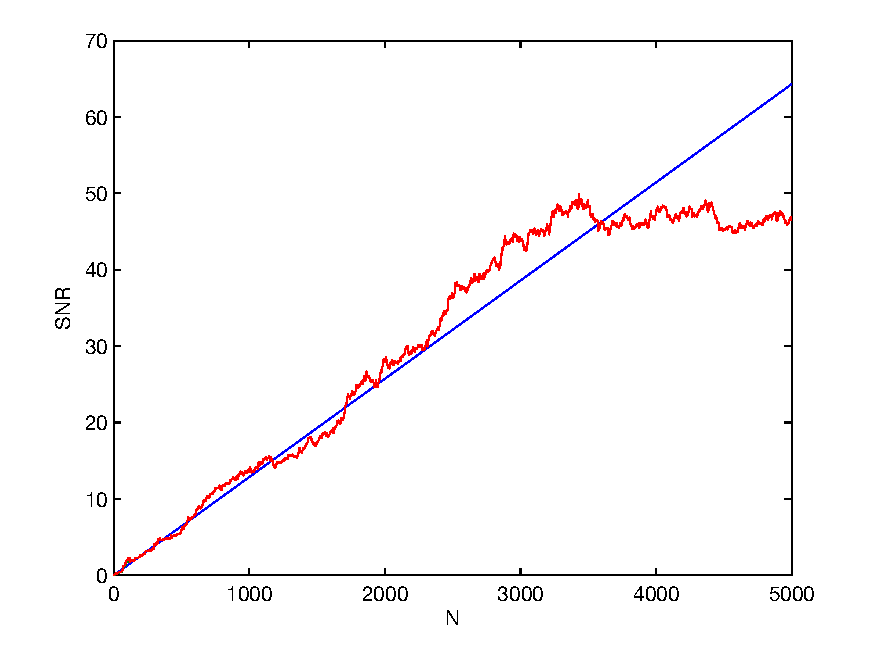
\includegraphics[width=12cm]{figure-ghost-snr.pdf}}
\caption{Theoretical (blue) and experimental (red) signal-to-noise ratio curves for a simple square transmission mask as a function of the number of realizations $N$.}
\label{figure:ghost-snr}
\end{figure}

\begin{figure}[htb]
\centerline{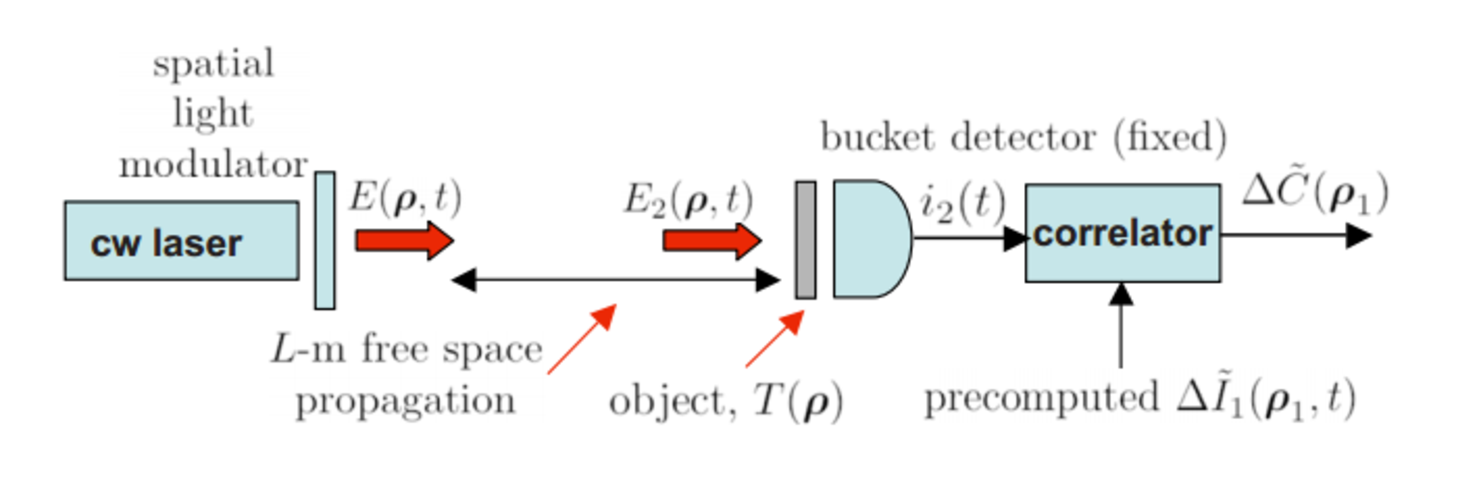
\includegraphics[width=12cm]{figure-ghost-computational-schematic.pdf}}
\caption{Computational ghost imaging schematic, in which there are no spatially resolving detectors and the reference arm is replaced by a computer-generated reference that is used to drive the spatial light modulator.}
\label{figure:ghost-computational-schematic}
\end{figure}

\section{Computational ghost imaging}

The pseudothermal and SPDC-generated signal and idler fields exhibit true randomness. However, SLM-based ghost imaging uses deterministic, pseudorandom modulations imposed by a computer. Since ghost imaging is a product of classical coherence propagation \cite{erkmen-unified}, we can in principle eliminate the reference arm altogether, in SLM-based ghost imaging, and replace it with a computational simulation of the free-space optical propagation from the SLM plane to the CCD camera plane, as proposed by Shapiro \cite{shapiro-computational,erkmen-from}. As shown in Figure \ref{figure:ghost-computational-schematic}, this computational replacement permits us to image an object using only a signal arm, without any spatially-resolving detectors.

\begin{figure}[t]
\begin{center}
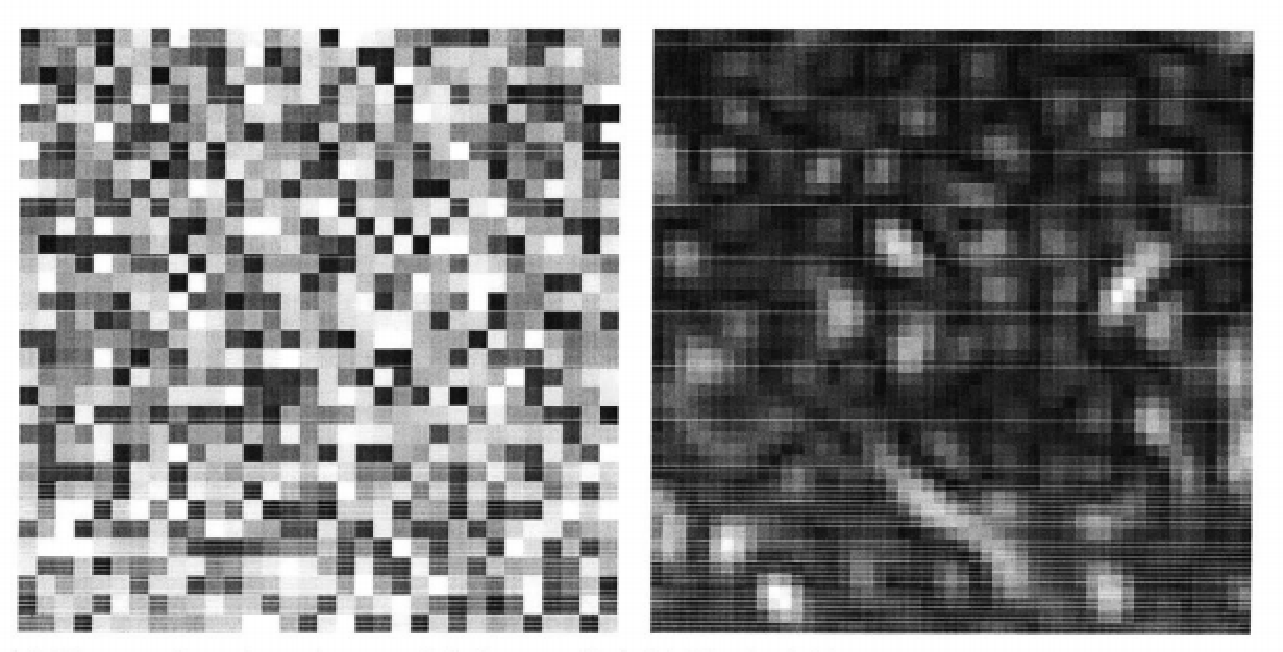
\includegraphics[width=13cm]{figure-ghost-slm-speckle.pdf}
\caption{(a) Sample pseudorandom phase pattern imposed on SLM. The phase modulation at each pixel is independent and uniformly distributed on $\left[0, 2\pi \right]$ and encoded as a gray-scale value in this visualization. (b) Simulated result of the far-field speckle pattern.}
\label{figure:ghost-slm-speckle}
\end{center}
\end{figure}

In order to realize this simulation, we consider the source field $E_R(\rho, t)$ at the SLM plane of the hypothetical reference arm, which is a product of the original cw laser beam field and the phases that would have been deterministically imposed on the reference arm SLM. In the case of phase-insensitive ghost imaging, these would be identical to the phases imposed on the signal arm; in the case of phase-sensitive ghost imaging, they would be the negative of those phases. We assume the SLM to be a square of size $D \times D$, with square pixels of size $d \times d$. Since $d$ is much smaller than the beam waist at the SLM, the light field can be approximated over each pixel as a plane wave. The sum of these plane waves at pixels indexed by $n = \left\{1 ... (D/d)^2\right\}$, multiplied by the phases $\phi_n(t)$ deterministically imposed on them, yields an SLM-plane field

\begin{equation}
E_R(\rho, t) = \sum_n \operatorname{rect}\left(\frac{x-x_n}{d}\right) \operatorname{rect}\left(\frac{y-y_n}{d}\right) e^{i\phi_n(t)}\,\,,
\end{equation}

where $\operatorname{rect}(\cdot)$ is the unit-length rectangle function and $\rho_n = (x_n,y_n)$ is the center of pixel $n$. We assume quasimonochromatic paraxial diffraction over a free-space path of length $L$ between the SLM and the CCD of the reference arm, which yields a CCD-plane field $E'$ given by \cite{hardy-thesis}:

\begin{equation}
E_R'(\rho', t) = \sum_n \frac{d}{\lambda_0 L} \operatorname{sinc}\left(\frac{x'd}{\lambda_0 L}\right) \operatorname{sinc}\left(\frac{y'd}{\lambda_0 L}\right) e^{-i k_0(x'x_n + y'y_n)/L} e^{-ik_0(|x'|^2 + |y'|^2)/2L} e^{i\phi_n(t)}\,\,.
\end{equation}


\begin{figure}[t]
\begin{center}
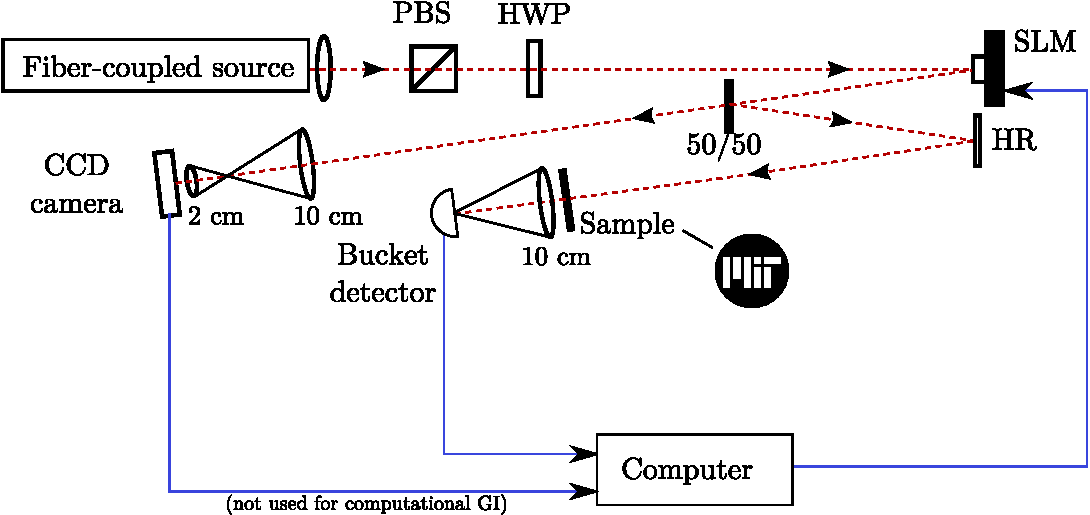
\includegraphics[width=13cm]{figure-ghost-computational-setup.pdf}
\caption{Pseudothermal, phase-insensitive ghost imaging setup used to test computational and compressed ghost imaging. In computational ghost imaging, we do not use the CCD camera.}
\label{figure:ghost-computational-setup}
\end{center}
\end{figure}


The far-field intensity pattern that would have been recorded by the reference arm CCD is then given by $I'(\rho, t) \propto |E'(\rho, t)|^2$. Figure \ref{figure:ghost-slm-speckle} shows a sample pseudorandom phase pattern with independent phase values each uniformly distributed over $[0, 2\pi]$, and the resulting computed far-field intensity pattern, which shows a speckle pattern with a feature size on the order of $\rho_L$.

We tested computational ghost imaging by first switching to a phase-insensitive ghost imaging setup using a single SLM and a beam splitter, as shown in Figure \ref{figure:ghost-computational-setup}. This eliminated any differences between the behaviors of two SLM devices. We performed computational ghost imaging in a fashion similar to traditional ghost imaging, using the computed far-field intensity pattern in place of a CCD image in the reference arm. In Figure \ref{figure:ghost-computational-result} we show side-by-side results of traditional ghost imaging and computational ghost imaging, realized over 9600 pseudorandom phase patterns, noting that the speed of image formation is similar in both cases. Bromberg et al. \cite{bromberg-ghost} also performed a similar experiment which demonstrated high-quality images with SNRs on par with theory for 16000 realizations.

\begin{figure}[t]
\begin{center}
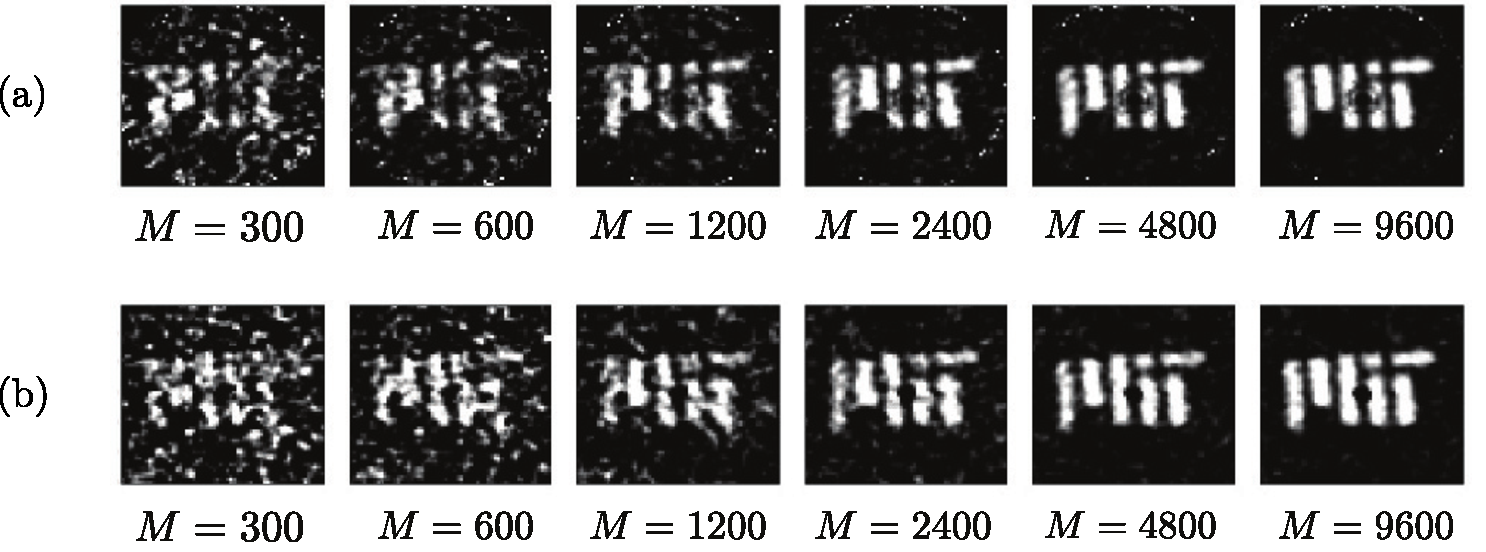
\includegraphics[width=16cm]{figure-ghost-computational-result.pdf}
\caption{Side-by-side results of an MIT logo mask imaged using (a) traditional ghost imaging with optical signal and reference arms and (b) computational ghost imaging in which the reference arm is replaced by a computer simulation, averaged over $M = 300$ to $9600$ independent pseudorandom phase patterns.}
\label{figure:ghost-computational-result}
\end{center}
\end{figure}

By replacing the reference arm with a computer simulation and using only a single bucket detector in the signal arm to obtain almost identical results, we verified that pseudothermal ghost imaging relies on simple classical coherence propagation, and not non-local quantum correlations as previously suggested in \cite{scarcelli-can}.

Although not explored significantly in this research, computational ghost imaging can provide a number of advantages over traditional ghost imaging. First, the elimination of the reference arm allows for a simpler device. Second, computational ghost imaging can be used to image objects at wavelengths for which bucket detectors are available but CCD arrays are not. Third, the intensity patterns can be simultaneously computed at multiple depths for a single phase pattern, allowing depth-of-field effects to be exploited to gain some degree of range resolution. These advantages are discussed in detail in \cite{erkmen-from}.

\section{Compressed ghost imaging}

We now reinstate the experimental reference arm in Figure \ref{figure:ghost-setup} and consider another variation of ghost imaging, in which we focus on the processing of our results to significantly reduce the required acquisition time. In this section we make use of compressed sensing (CS) \cite{candes-stable}, a novel processing technique which has been applied to numerous fields of imaging, notably single-pixel cameras \cite{duarte-single}, whose setups are very similar in nature to signal arm of a ghost imaging setup. Katz et al. first implemented compressive ghost imaging using a rotating ground glass and a beamsplitter \cite{katz-compressive}; here we attempt to apply a similar technique to SLM-based ghost imaging.

\begin{figure}[t]
\begin{center}
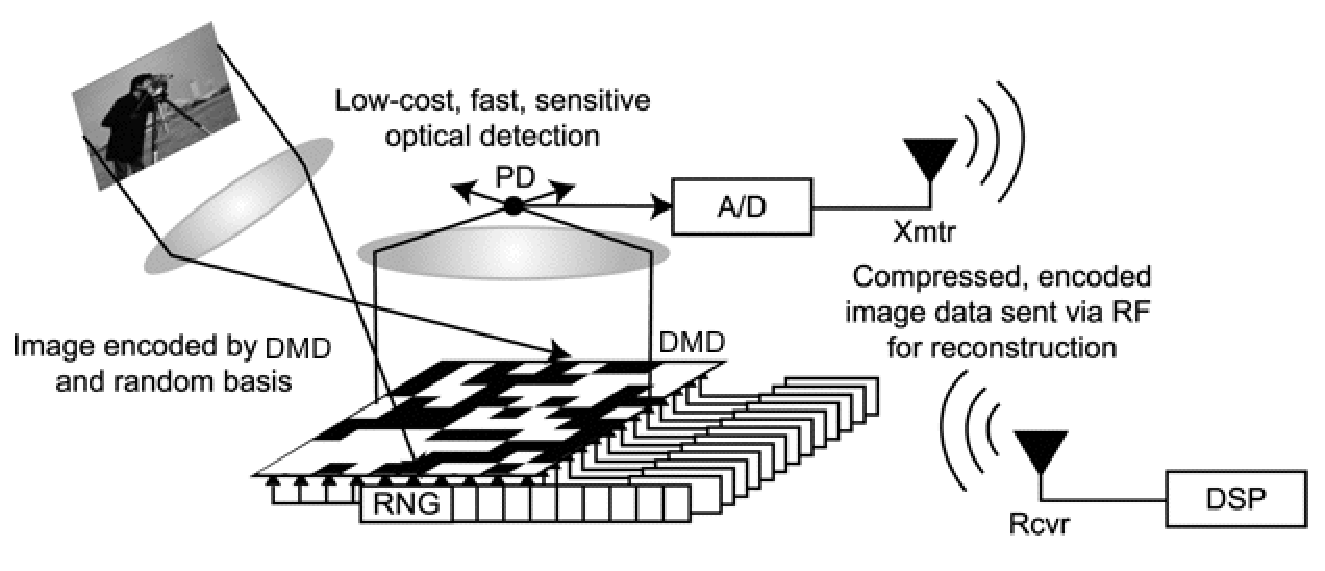
\includegraphics[width=14cm]{figure-ghost-cscam.pdf}
\caption{Schematic of the Rice University single pixel camera, reproduced from \cite{takhar-new}. DMD: digital micromirror device, PD: photodetector, DSP: digital signal processor, RNG: random number generator. (TODO: add (a) and (b) to figure)}
\label{figure:ghost-cscam}
\end{center}
\end{figure}

The basic idea behind compressed sensing is that given that real-world objects exhibit some degree of spatial structure, a small number of measurements of known, random linear projections of the object contains enough information to reconstruct the object. This spatial structure is captured by sparsity in some transform basis, such as the discrete cosine transform (DCT) or wavelet basis. In other words, we expect that most real-world objects have a relatively small number of nonzero coefficients in the transform basis.

Making this very realistic assumption drastically reduces our solution space, and consequently the number of measurements required for faithful reconstruction, a method first proposed by Candes et al. \cite{candes-stable}. Rather than using averaging to slowly converge toward our solution over thousands of realizations, we instead use a relatively low number of measurements, treat the image as a solution to an underdetermined linear system, and employ computational optimization techniques to move to a solution that fits our sparsity criteria. Sparsity is usually quantified in terms of the $\ell_1$-norm (sum of the absolute values) of the coefficients in the transform basis \cite{candes-stable}, which allows us to employ well-known, efficient convex optimization algorithms to quickly search for a global optimum.

Compressed sensing was used by the single-pixel camera at Rice University \cite{duarte-single}, as shown in Figure \ref{figure:ghost-cscam}. The single-pixel camera uses a digital micromirror device (DMD), whose pixels can be set to selectively reflect light, placed at the image plane of a camera, and a single-pixel photodetector to collect all the light reflected by the DMD. Although their implementation placed the DMD at the receiver, allowing it to be used with arbitray illumination sources, the single-pixel camera could in principle be accomplished by using a custom, broadband light source and spatially modulating the illumination using the DMD (i.e. projecting known illumination patterns onto the object).

This operation of the single-pixel camera is functionally similar to ghost imaging in that a pseudorandom spatial pattern is projected onto the object and the single-pixel detector is equivalent to a bucket detector. The only difference relevant to data processing is that in ghost imaging, we are unable to arbitrarily conFigure the intensity pattern at the object plane; we can only conFigure the phase modulations at the SLM and determine the resulting far-field intensity pattern at the object plane either experimentally (using a reference arm) or by simulation (using computational ghost imaging). However, as long as we have knowledge of these patterns, we can employ the compressed sensing technique that is associated with single-pixel cameras.

To computationally reconstruct a $N \times N$-pixel image $x_{i \in [0,N^2]}$, we solve for
\begin{equation}
\hat{x} = \underset{x}{\operatorname{arg\,min}}\,\,||W\{x\}||_1,\,\,\, \operatorname{s.t.}\,Ax = b
\end{equation}
where $x$ is a $1$-by-$N^2$ vector representing the pixels of the image rearranged as a single column, $A$ is a $M$-by-$N^2$ matrix containing $M \ll N^2$ realizations of object-plane intensity patterns, one pattern per row and rearranged in the same order as $x$, $b$ is a $M$-by-1 vector that stores the resulting bucket detector measurements for each pattern, and $W\{\cdot\}$ is a sparsifying transform (such as DCT, for example). Assuming the system operates perfectly and delivers the correct observations for $b$, this equation determines the sparsest solution $x$ that satisfies the underdetermined equation system $Ax = b$.

\begin{figure}[t]
\begin{center}
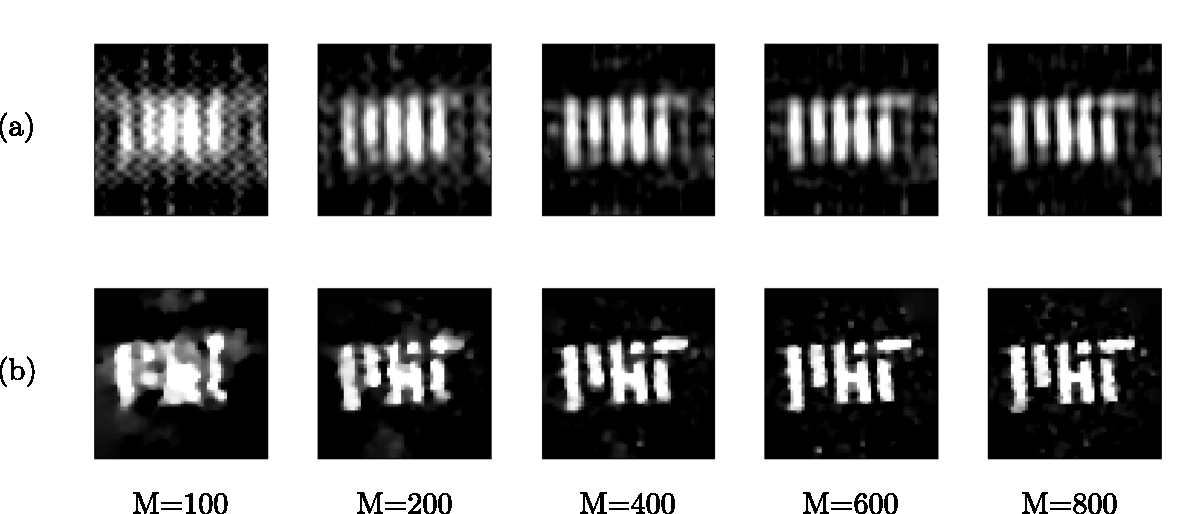
\includegraphics[width=16cm]{figure-ghost-compressed-dctvstv.pdf}
\caption{Ghost images processed using compressed sensing for a binary MIT logo mask, using (a) DCT and (b) TV sparsifying transforms.}
\label{figure:ghost-compressed-dctvstv}
\end{center}
\end{figure}


However, since $b$ will be corrupted by noise, in most experimental situations it is necessary to relax this equality constraint. We do this by solving instead for
\begin{equation}
\hat{x} = \underset{x}{\operatorname{arg\,min}}\,\,||W\{x\}||_1,\,\,\, \operatorname{s.t.}\,||Ax - b||_2<\epsilon
\end{equation}
where $\epsilon$ represents the maximum magnitude of the error in the bucket detector measurements. This optimization problem can be solved efficiently using convex optimization techniques. We make use of the L1-Magic \cite{l1magic} package for MATLAB which is designed specifically to solve this problem. Another similar method to relax the equality constraint is to solve for
\begin{equation}
\hat{x} = \underset{x}{\operatorname{arg\,min}}\,\,\left[\,||W\{x\}||_1\,\,+\,\,\frac{1}{2\rho}||Ax - b||_2^2\,\right]
\end{equation}
for a tunable relaxation parameter $\rho$ which can be solved using the YALL1 package \cite{yall1} developed at Rice University.

\begin{figure}[t]
\begin{center}
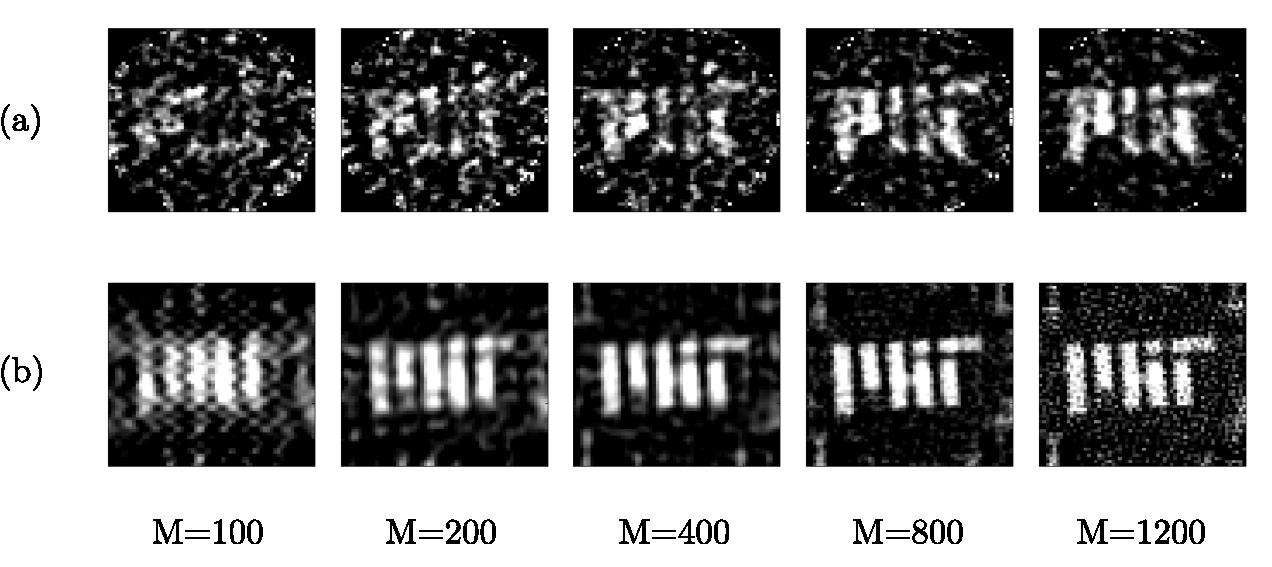
\includegraphics[width=16cm]{figure-ghost-compressed-bszl1.pdf}
\caption{Ghost images of an MIT logo mask imaged using (a) traditional averaging and (b) compressed sensing using the same data set.}
\label{figure:ghost-compressed-bszl1}
\end{center}
\end{figure}

\begin{figure}[h]
\begin{center}
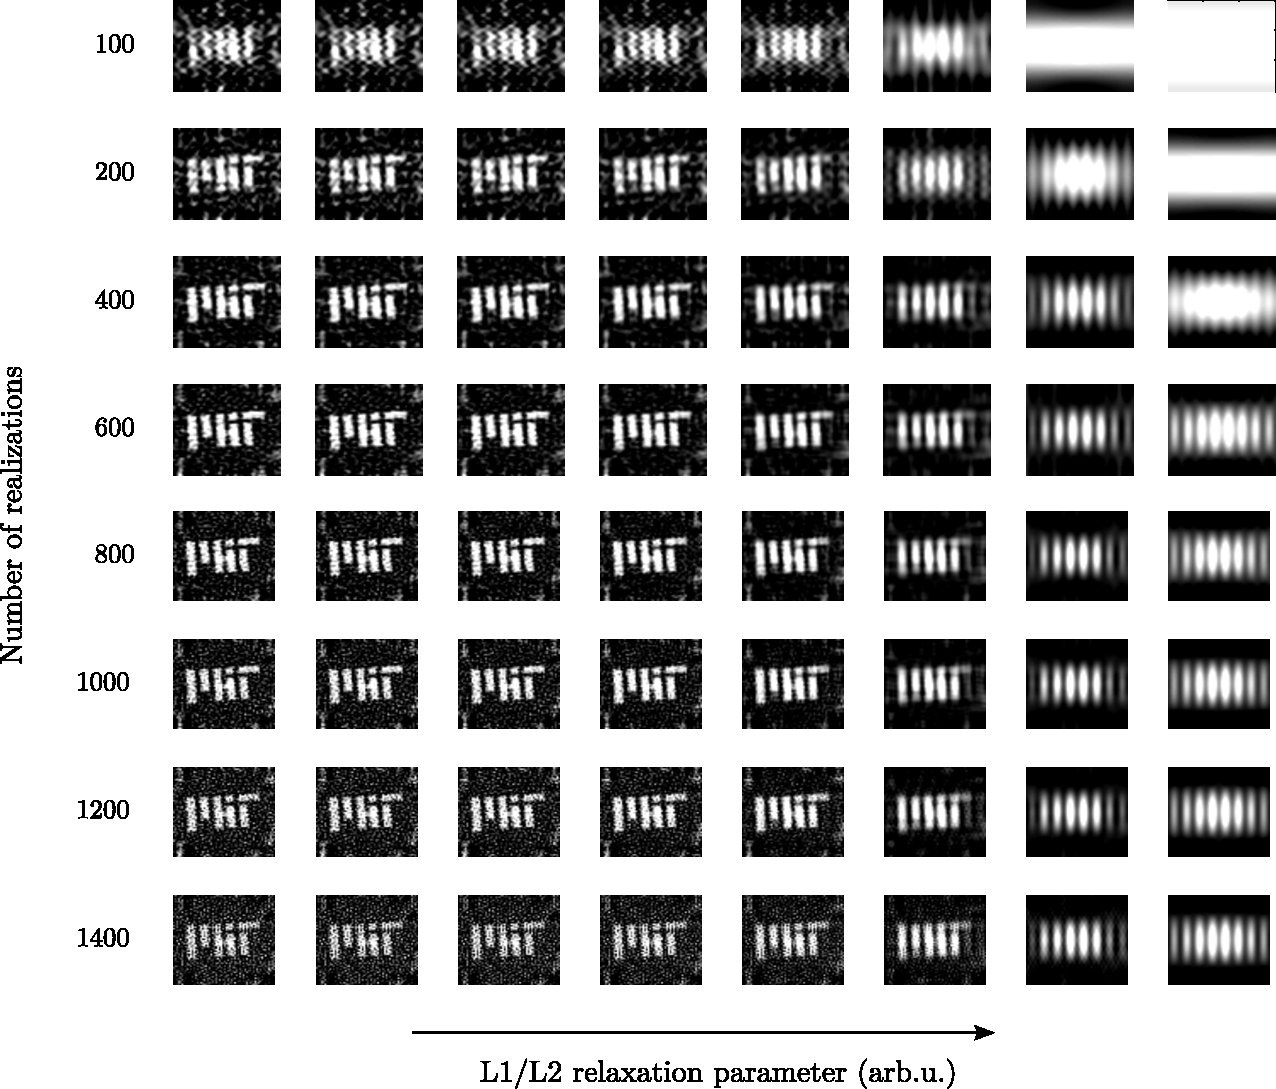
\includegraphics[width=16cm]{figure-ghost-compressed-tuning.pdf}
\caption{Relaxing the constraint to varying degrees in the computational reconstruction using DCT as a sparsifying basis. From top to bottom, we increase the number of realizations, and from left to right, we relax the equality constraint, allowing for errors in the data. We used this process to determine the value of the relaxation parameter $\epsilon$ to use.}
\label{figure:ghost-compressed-tuning}
\end{center}
\end{figure}

We use the same phase-insensitive ghost imaging setup shown in Figure \ref{figure:ghost-setup} and the same transmission mask of the MIT logo. Since this is a binary mask with sharp edges, we note that DCT may not be a suitable sparsifying basis because it is not localized in space and the sharp edges would excite numerous basis components. A more suitable sparsifying transform for this type of sample is based on total variation (TV), in which we solve for
\begin{equation}
\hat{x} = \underset{x}{\operatorname{arg\,min}}\,\,||\operatorname{TV}\left(x\right)||_1,\,\,\, \operatorname{s.t.}\,||Ax - b||_2<\epsilon
\end{equation}
where TV$\left(\cdot\right)$ represents the sum of the absolute differences of consecutive pixels in the image. This problem is also readily solved by L1-Magic \cite{l1magic}. Figure \ref{figure:ghost-compressed-dctvstv} shows results of ghost imaging using compressed sensing using DCT and TV sparsifying transforms, showing that TV does indeed perform better for this particular type of mask. In both cases, we scan over the relaxation parameter $\epsilon$ to find an optimal value, as illustrated in \ref{figure:ghost-compressed-tuning} for the DCT case. If the constraint is too tight, artifacts originating from noise remaining in the image; if the constraint is too loose, the convex optimization routine over-smoothes the image and arrives at a solution that does not fit the data.

We also compare compressed sensing to traditional ghost image processing based on the second-order cross-correlations between the reference and bucket signals. Figure \ref{figure:ghost-compressed-bszl1} shows side-by-side results of ghost images obtained using traditional averaging and TV compressed sensing using identical data sets. We see in this case that by 200 realizations, the image obtained by compressed sensing is already intelligible, and by 400 realizations it is clear. In contrast, the traditional averaging method is barely intelligible before 1200 realizations; in Figure \ref{figure:ghost-computational-result} of the previous section we observed that it took several thousand realizations to form a high-quality image.

\section{Computational compressed ghost imaging}

We now turn to the question of whether it is possible to entirely replace the reference arm with a computational simulation, and apply compressed sensing techniques at the same time. Figure \ref{figure:ghost-compressed-czl1} shows sample results of applying our compressed sensing algorithm to the data set used to produce computational ghost images in Figure \ref{figure:ghost-computational-result}. We see that although there is barely some evidence of an object, we are unable to extract a usable image from this method. We were, however, able to recover images for simpler masks, as seen in Figure \ref{figure:ghost-ccgi}.

In order to debug this issue further, in Figure \ref{figure:ghost-slm-samples} we reinstate the physical reference arm and compare images obtained by the CCD with our computational simulation; we see a significant discrepancy in the two patterns. We attribute this largely to imperfections in the SLM as described earlier in the Pitfalls section. In particular, since the effect of a single SLM pixel on the far-field speckle pattern is not localized, we expect that the deviations in the flatness of the SLM plane may highly affect the far-field pattern. In addition, we are unable to reliably predict the physical behavior of the dead space regions of our SLM. In the case of computational ghost imaging without compressed sensing, most of these discrepancies are averaged away after a large number of realizations. However, compressed sensing searches for a sparse object given an underdetermined set of data rather than averaging over a long time, making it much less tolerant to systematic errors; it is essential that especially the measurement matrix ($A$) be sufficiently accurate, which as demonstrated by Figure \ref{figure:ghost-slm-samples} is not the case.

\begin{figure}[t]
\begin{center}
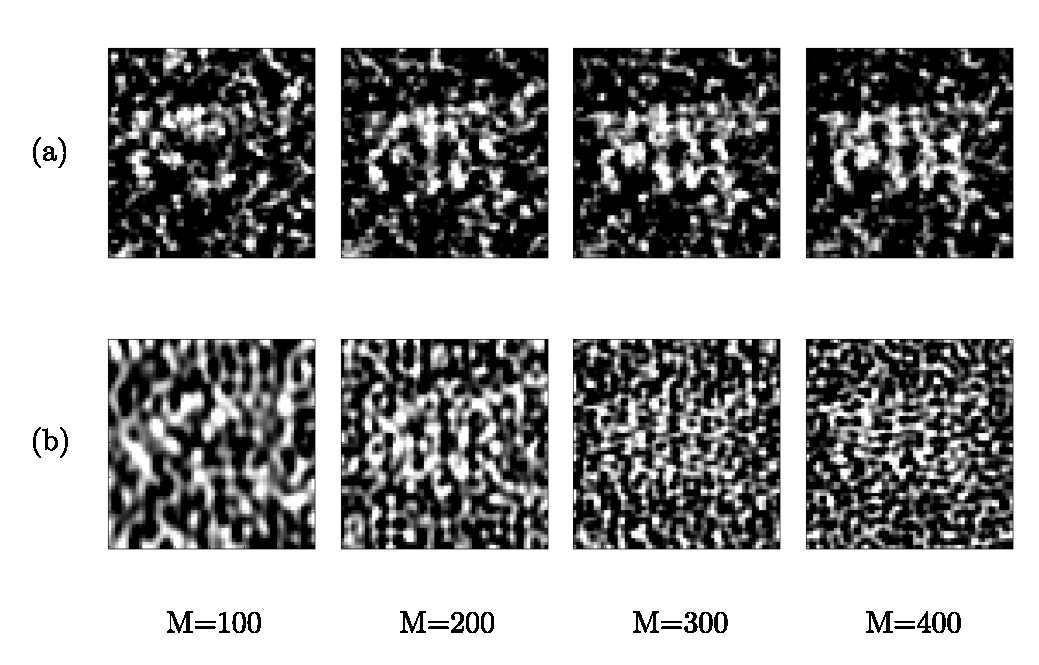
\includegraphics[width=13cm]{figure-ghost-compressed-czl1.pdf}
\caption{Attempts to obtain images of an MIT logo mask imaged using compressed sensing with a computationally-simulated refererence arm. (a) shows the computational ghost imaging result using traditional processing, and (b) shows the result of applying compressed sensing techniques. (TODO: add (a) and (b) to figure)}
\label{figure:ghost-compressed-czl1}
\end{center}
\end{figure}

\begin{figure}[t]
\begin{center}
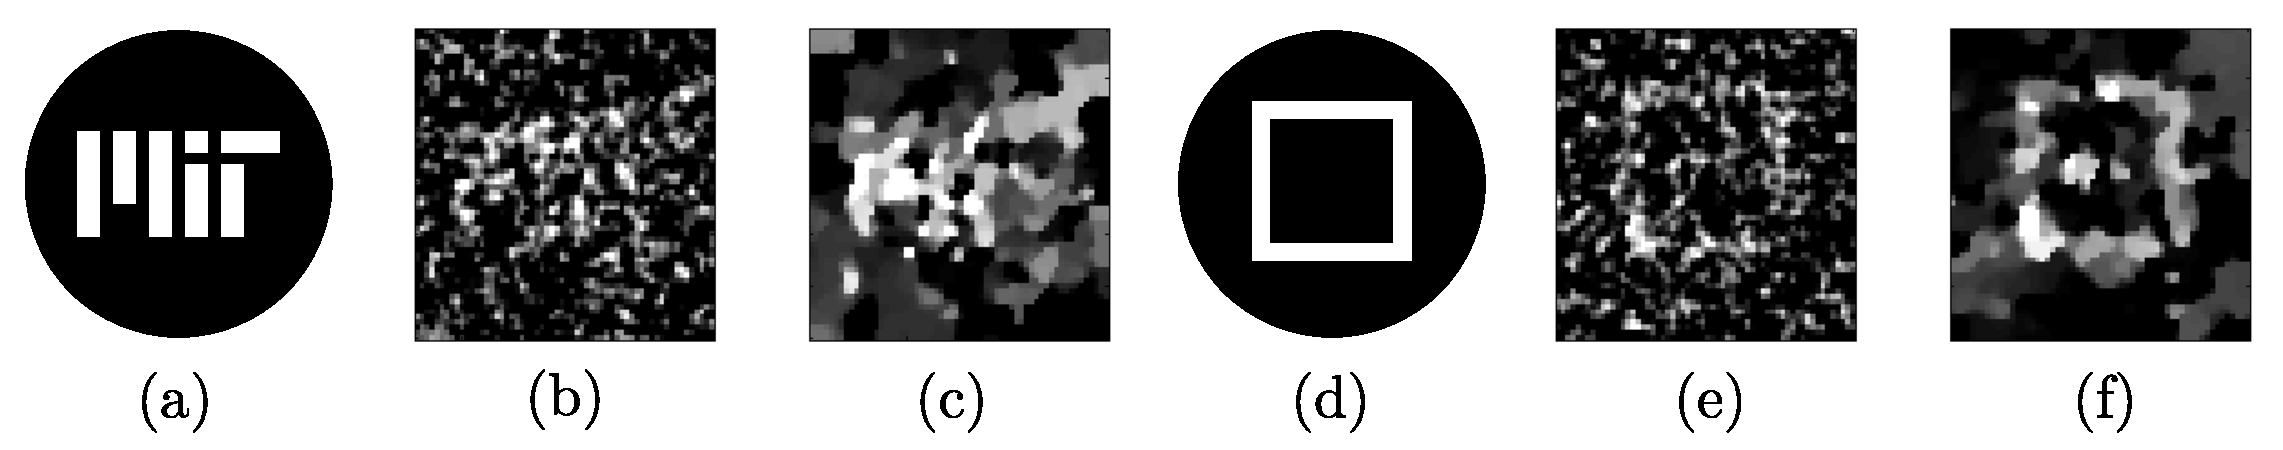
\includegraphics[width=15cm]{figure-ghost-ccgi.pdf}
\caption{Computational compressed ghost imaging using a simpler object. (a) MIT logo mask and ghost image results for (b) covariance-based and (c) compressed sensing using TV minimization for the same number of realizations, showing the same problems seen in Figure \ref{figure:ghost-compressed-czl1}. (d) Simpler square mask and results using (e) covariance-based and (f) compressed sensing using TV minimization.}
\label{figure:ghost-ccgi}
\end{center}
\end{figure}

\begin{figure}[h]
\begin{center}
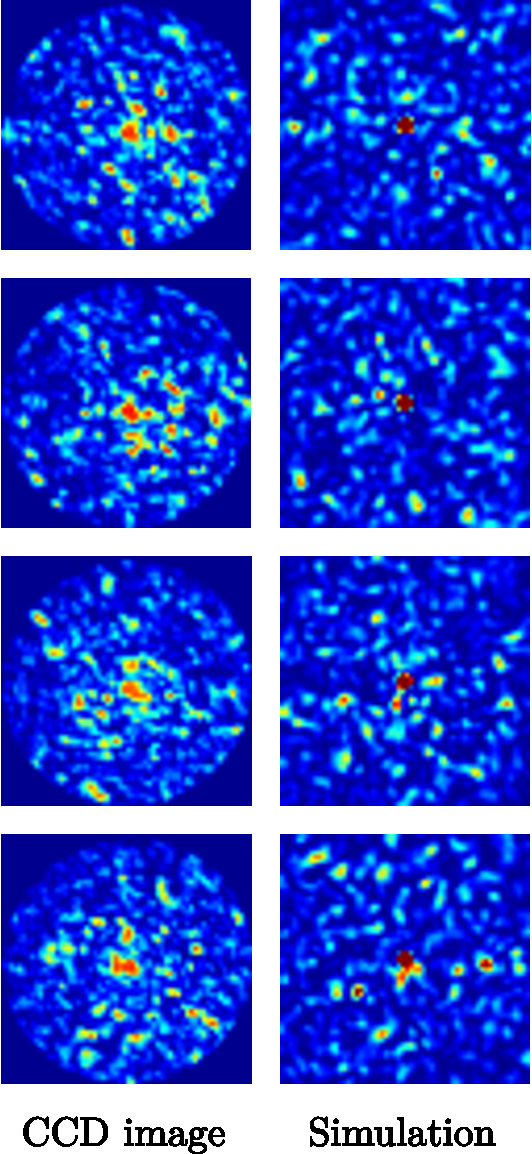
\includegraphics[height=20cm]{figure-ghost-slm-samples.pdf}
\caption{Sample speckle patterns acquired by a CCD array (left) and the corresponding computational simulation results (right). We attribute the large discrepancy to imperfections in the SLM array.}
\label{figure:ghost-slm-samples}
\end{center}
\end{figure}

\section{Conclusions}

Similar to our work with phase-coherent optical coherence tomography described in the previous chapter, we present phase-sensitive far-field ghost imaging, another example of an experiment previously thought to be exclusive to quantum sources. In addition, we present a new type of classical phase-sensitive light source that is realized by deterministically imposing pseudorandom phase patterns on a pair of light beams using spatial light modulators. We also demonstrate that much like biphoton ghost imaging, phase-sensitive classical ghost imaging also produces an inverted image in the far field.

We demonstrate a couple of advantages that are unique to classical ghost imaging. First, since we impose deterministic phase patterns, we can eliminate the reference arm from the experiment entirely and replace it with a computer simulation. This also greatly simplifies the setup and allows it to be potentially used for long-range ghost imaging where a physical reference arm would be impractical to imprement, or imaging at wavelengths where bucket detectors are available but CCD arrays are not. Such a simulation would not be possible using quantum light sources. Similar to our PC-OCT experiment described in the previous chapter, our use of classical detectors permits us to operate at much higher power levels and improve acquisition speed. In contrast to quantum ghost imaging experiments which often require hours or more of acquisition time, we were able to obtain clean images within a few minutes with our main limitation being only the SLM frame rate, offering a practical speedup by several hundred times.

We additionally recognize that our imaging targets have spatial structure and are far from pixelwise random in nature. This is captured by the concept of spatial sparsity, and explore the use of compressed sensing to further speeding up the acquisition time by computationally reconstructing the image instead of averaging over a large number of trials. We show that with as few as 400 realizations we obtain clear images of our transmission mask, offering a factor of 5-10 speedup in acquisition in comparison with traditional averaging methods.

We also explored the possibility of combining computational ghost imaging with compressed sensing, which did not yield good results in our case. We attribute this to deficiencies in our SLM which prevent us from accurately simulating its physics, which is not essential for traditional acquisition which averages out such errors, but negatively affects compressed sensing which requires an accurate model of the measurement being performed. 
